\section{Background and definitions}
We first review the relevant background on model evaluation and issues caused by partial labeling. 

%%%%%%%%%%%%%%%%%%%%%%%%%%%%%%%%%%%%%%%%%%%%%%%%
%%%
%		RANK DISTRIBUTIONS

%%%
%%%%%%%%%%%%%%%%%%%%%%%%%%%%%%%%%%%%%%%%%%%%%%%%

\subsection{Rank distributions and contingency tables} \label{contingency-intro}
%Many classifiers assign each example a numeric \emph{decision value} during prediction. This is a measure of confidence that the instance belongs to the positive class, e.g. logistic regression yields the associated probability ($\hat{y}\in [0, 1]$) and SVM classifiers yield a signed distance to the separating hyperplane ($\hat{y} \in \mathbb{R}$). Any binary classifier can be described as a functional $\mathcal{C}$ that maps input vectors $\mathbf{x}\sim\inputspace$ onto the real line, i.e. $\mathcal{C}:\inputspace \mapsto \mathbb{R}$. Higher decision values imply higher confidence that the instance belongs to the positive class. 

We focus on binary decision problems, where the goal is to classify examples as either positive or negative. Most learned models (e.g., SVM, logistic regression, naive Bayes) predict a numeric score for each example where higher values imply higher confidence that the instance belongs to the positive class. Typically, a \emph{ranking} $\overall$ is produced by sorting examples in descending order by their numeric score such that confident positive predictions are ranked close to the top of $\overall$.\footnote{Which means a low value for rank in this work, though this is often referred to as \emph{highly ranked} in literature.}  

%$\rank(\overall, x)$ denotes the rank of an instance $x$ in $\overall$.


%\emph{decision value} to each example during prediction. Intuitively, the decision value represents the confidence that the instance belongs to the positive class. Typically, higher decision values imply higher confidence that the instance belongs to the positive class. 


 %The rank of an instance is defined by its position in $\overall$, such that confident positive predictions (characterized by high decision values) are ranked close to the top of $\overall$.\footnote{Which means a low value for rank in this work, though this is often referred to as \emph{highly ranked} in literature.}

Within a ranking $\overall$, we treat $\pos \subset \overall$ as the subset of examples with positive labels, $\bar{\pos} = \overall - \pos$  as the subset of examples with negative labels, and let $\rank(\overall, x)$ denote the rank of an instance $x$ in $\overall$.  Given a cutoff rank $r,$ predictions can be made by assigning the positive class to the $r$ top ranked instances and the negative class to the rest. This decision rule yields a \emph{true positive rate (TPR)}, which is the fraction of positive examples that are correctly labeled as positive, and \emph{false positive rate (FPR)}, which is the fraction of negative examples that are incorrectly labeled as positive:
\begin{align}
\TPR(\pos, r) &= \probability(\rank(\overall, x) \leq r\ |\ x \in \pos), \nonumber \\
	      &= |\{\ x \in \pos\ :\ \rank(\overall, x) \leq r\}|\ /\ |\pos|, \label{tpr-def} \\
\FPR(\pos, r) &= \probability(\rank(\overall, \bar{x}) \leq r\ |\ \bar{x} \in \bar{\pos}) = \TPR(\overall - \pos, r). \label{fpr-def}
\end{align}
\noindent Given the number of positives $|\pos|$ and negatives $|\overall-\pos|$, the contingency table for a rank $r$ is: \\
\begin{minipage}[c]{0.45\textwidth}
\begin{align}
\TP(\pos,r) &= \TPR(\pos, r) \cdot |\pos|, \label{tp-def} \\
\FN(\pos,r) &= |\pos| - \TP(\pos, r), 
\end{align}
\end{minipage}\hfill\begin{minipage}[c]{0.52\textwidth}
\begin{align}
\FP(\pos,r) &= \FPR(\pos, r) \cdot |\overall-\pos|, \nonumber \\
\TN(\pos,r) &= |\overall-\pos| - \FP(\pos,r). %= (1 - \FPR(\pos, r)) \cdot |\overall - \pos| \\
\end{align}
\end{minipage}

The rank distribution of a set of instances $\pos$ within an overall ranking $\overall$ is defined as the distribution of their corresponding ranks within $\overall$. The rank cumulative distribution function (CDF) of a set of instances $\pos$ is defined as the (empirical) CDF of their ranks, i.e. $\forall\ r \in \{1,\ldots,|\overall|\}$:
\begin{equation}
\cdf{\pos}{r} = \probability(\rank(\overall, x) \leq r \ |\ x \in \pos). \label{rankcdf}
\end{equation}
The concept of rank CDF is illustrated in Figure~\ref{fig:rank-cdf}. Note that $ \cdf{\pos}{r} \equiv \TPR(\pos, r) $ (Equations~\eqref{tpr-def} and~\eqref{rankcdf}), that is, the rank CDF of the set of positives $\pos$ at rank $r$ in an overall ranking $\overall$ can be interpreted directly as a true positive rate, when labeling the $r$ top ranked instances as positive.
%%%%%%%%% HACK TO MAKE EVERYTHING FIT %%%%%%%%
%%%%%%%%%%%%%%%%% END OF HACK %%%%%%%%%%%%%%%%
\begin{figure}[ht]
  \centering
  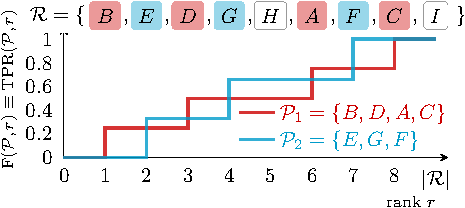
\includegraphics[width=0.6\textwidth]{rank-cdf.pdf}
  \caption{Rank CDF of two sets of positives $\pos_1 = \{B, D, A, C\}$ and $\pos_2=\{E, G, F\}$ within an overall ranking $\overall=\{B,E,D,G,H,A,F,C,I\}$, with $|\pos_1|=4$ and $|\pos_2|=3$. In practice $\overall$ is obtained by sorting the data according to classifier score. The rank CDF of a set $\mathcal{S}\subseteq \mathcal{R}$ is based on the positions of elements of $\mathcal{S}$ in $\overall$. } 
  \label{fig:rank-cdf}
\end{figure}

We use two convenience functions to partition sets of ranks:
\begin{align*}
\topfun(X, \ranksymb) &= \{\ \rank(\overall, x) \leq \ranksymb\ :\ x \in X\ \}, \\
\bottomfun(X, \ranksymb) &= \{\ \rank(\overall, x) > \ranksymb\ :\ x \in X\ \},
\end{align*}
such that $\topfun(X,\ranksymb)\ \cup\ \bottomfun(X,\ranksymb) = X$ and $|\topfun(X,r)| = \cdf{X}{\ranksymb}\cdot |X|$. 

%%%%%%%%%%%%%%%%%%%%%%%%%%%%%%%%%%%%%%%%%%%%%%%%
%%%
%		ROC CURVES
%%%
%%%%%%%%%%%%%%%%%%%%%%%%%%%%%%%%%%%%%%%%%%%%%%%%

\subsection{ROC and PR curves} \label{roc}
Receiver operator characteristic (ROC) curves are used extensively for evaluating classifiers in machine learning \citep{Bradley:1997:UAU:1746432.1746434} as they illustrate the performance of a model over its entire operating range. ROC curves depict how a model's true positive rate (shown on the y-axis) varies as a function of its false positive rate (shown on the x-axis). Each cutoff rank $r \in \{1,\ldots,|\overall|\}$ corresponds to a single point (i.e., (FPR, TPR) pair) in ROC space (Eqs.~\eqref{tpr-def} and \eqref{fpr-def}). An (empirical) ROC curve for a ranking $\overall$ and set of positives $\pos \subset \overall$ is constructed by computing $\FPR(\pos, r)$ and $\TPR(\pos, r)$ at each rank $r$ and interpolating by drawing a straight line between points corresponding to consecutive ranks.  
The area under an ROC curve (AUROC) is a commonly used summary statistic, typically ranging between $0.5$ (random model) and $1$ (perfect model). AUROC is a popular  criterion in model selection and is often used as the optimization objective in hyperparameter search \citep{Bradley:1997:UAU:1746432.1746434}.

%ROC curves are insensitive to changes in the distribtuion of because FPR and TPR are each based on a single column of a contingency table \citep{fawcett2006introduction}. ROC curves can also be used for cost-sensitive learning \citep{provost1997analysis}. %and can be used for cost-sensitive learning.

%The area under an ROC curve (AUROC) is a commonly used summary statistic which typically ranges between $0.5$ (random model) and $1$ (perfect model). AUROC is equal to the probability that a random positive is ranked higher than a random negative, which is equivalent to the Wilcoxon test of ranks \citep{hanley1982meaning}. It is a popular criterion to optimize during hyperparameter search \citep{lessmann2008benchmarking, DBLP:journals/corr/ClaesenSPMM14}.


Precision-Recall (PR) curves  \citep{davis2006relationship} are an alternative to ROC curves that show how a model's precision (y-axis) varies as a function of recall (x-axis). Recall is equivalent to TPR and precision is the fraction of examples classified as
positive that are truly positive ($\TP / (\TP+\FP)$). PR curves are widely used when there is a skew in the class distributions~\cite{davis-icml09,claesen2014robust}.



%Algorithm 2 has a clear advantage over Algorithm 1. This difference exists because in this domain the number of negative examples greatly exceeds the number of positives examples. Consequently, a large change in the number of false positives can lead to a small change in the false positive rate used in ROC analysis

%were originally used in information retrieval \citep{raghavan1989critical}. PR curves visualize the evolution of precision ($\TP / (\TP+\FN)$) versus recall (TPR) and can be used as an alternative to ROC curves to assess classifier performance.

%%%%%%%%%%%%%%%%%%%%%%%%%%%%%%%%%%%%%%%%%%%%%%%%
%%%
%		PARTIAL LABELING
%%%
%%%%%%%%%%%%%%%%%%%%%%%%%%%%%%%%%%%%%%%%%%%%%%%%

\subsection{Evaluation with partially labeled data}
In the partial labeling setting, $\overall$ consists of disjoint sets of known positives $\knownpos$, known negatives $\knownneg$ and unlabeled instances $\unlabeled$. %, i.e., $\overall = \knownpos \cup \knownneg \cup\ \unlabeled$.
The unlabeled set $\unlabeled$ consists of latent positives $\latentpos$ and latent negatives. The fraction of latent positives in the unlabeled set plays a crucial role in our work, denoted by $\beta$:
\begin{equation}
\pfrac = \probability(x \in \latentpos\ |\ x \in \unlabeled) = |\latentpos|\ /\ |\unlabeled|. \label{pfrac} %\frac{|\latentpos|}{|\unlabeled|}. \label{pfrac}
\end{equation}
%We assume an estimate $\hat{\pfrac} \approx \pfrac$ is available. This can be obtained via direct statistical estimates based on training data \citep{Elkan:2008:LCO:1401890.1401920} or domain knowledge, e.g. in disease screening $\hat{\pfrac}$ is the prevalence of undiagnosed patients of the disease \citep{holmberg1996estimated, rathmann2003high}.

Note that computing contingency tables requires fully labeled data. If only a few labeled instances of both classes are available, they can be used to compute rough estimates of predictive performance. However, if only positive labels are available, even a rough approximation of common metrics cannot be estimated directly as we do not know which unlabeled examples are positives and which are negative. A common approach to evaluate models in a PU learning context is to treat the full unlabeled set as negative \citep{mordelet2011prodige,sifrim2013extasy,sechidis2014statistical}, though we will show that this may lead to spurious results. 

%This approach is inherently pessimistic: at any cutoff rank, the FPR is overestimated and the TPR is underestimated because all latent positives are treated as negative. Hence, this method is only useful when $\pfrac$ is small, that is, $\pfrac < 0.01$ as its bias is related to $\pfrac/\hat{\pfrac}$. This is particularly problematic for PR curves, as we will show later. \todo{rewrite last 3 phrases}

%Trivial best and worst case bounds on performance are easily obtained by considering all latent positives to be ranked at the top or bottom of the unlabeled set, respectively. However, these are too wide for any meaningful use when $|\latentpos| \gg |\knownpos|$, which is a common situation in practice.

%We focus on the PU learning setting, in which only positive labels are available, i.e. $\knownneg = \emptyset$, though our approach can include known negatives too (incorporating known negatives is explained in Theorem~\ref{main-theorem} and Section~\ref{contingency}).

%Computing contingency tables and performance curves based on an overall ranking $\overall$ as described in Sections~\ref{contingency-intro} and \ref{roc} requires a known set of \emph{all} positives $\pos_\Omega = \knownpos \cup \latentpos$. Since $\latentpos$ is unknown, they cannot be computed directly. Section~\ref{rank-roc} details how to tackle this problem theoretically and Section~\ref{practical} describes a practical approach.



%\subsection{Performance curves from partially labeled data}
%If only a few labeled instances of both classes are available, they can be used to construct a rough estimate of either the ROC or PR curve. However, if only positive labels are available, even a rough approximation of the ROC or PR curve cannot be estimated directly. 

%In PU learning, a simple approach is to treat the full unlabeled set as negative, i.e., assume $\hat{\pfrac} = 0$. This approach is inherently pessimistic: at any cutoff rank, the FPR is overestimated and the TPR is underestimated because all latent positives are treated as negative. Hence, this method is only useful when $\pfrac$ is small, that is, $\pfrac < 0.01$ as its bias is related to $\pfrac/\hat{\pfrac}$. This is particularly problematic for PR curves, as we will show later.

%Trivial best and worst case bounds on performance are easily obtained by considering all latent positives to be ranked at the top or bottom of the unlabeled set, respectively. However, these are too wide for any meaningful use when $|\latentpos| \gg |\knownpos|$, which is a common situation in practice.
